173. \begin{figure}[ht!]
\center{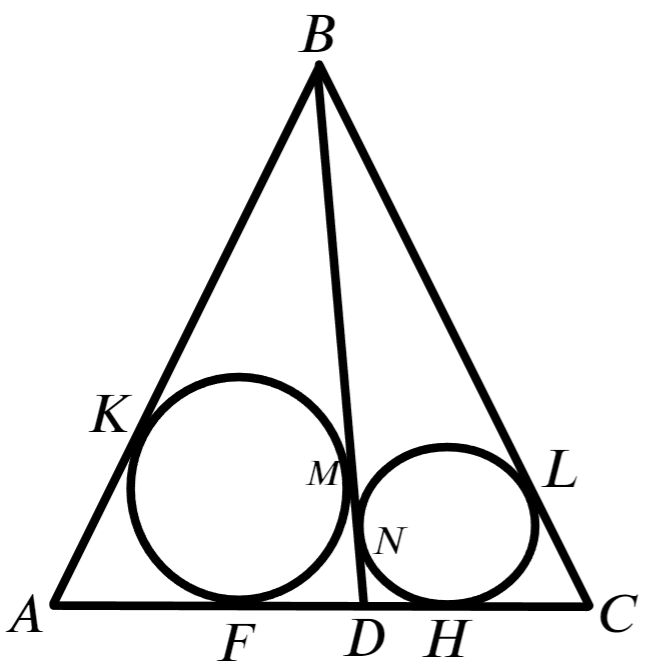
\includegraphics[scale=0.35]{g9-173.png}}
\end{figure}\\
Так как $AD>AC,$ точка $M$ находится между $B$ и $N.$ Отрезки касательных, проведённых из одной точки, равны, отсюда имеем равенства $BM = BK,\ BN = BL,\ AK =AF,\ CL = CH,\ DF = DM,\ DN = DH.$ Тогда $MN = BN - BM = BL - BK = (BC - LC) - (AB - AK) = AK - LC =
AF - HC = (AD-FD)-(CD-DH) = DH - FD+2 = DN - DM +2 =2 -MN \Rightarrow 2MN = 2,\ MN=1.$\\
